% Copyright 2020 Glen Newton
% License: Creative Commons Attribution-ShareAlike 4.0 International License https://creativecommons.org/licenses/by-sa/4.0/legalcode
%\documentclass[a0paper,10pt]{article}
\documentclass[12pt]{article}


\usepackage{tikz}
\usepackage[margin=6mm]{geometry}

\usepackage[extreme]{savetrees}
\usepackage{microtype}
\usepackage[hidelinks]{hyperref}
\usetikzlibrary{mindmap,positioning}

%\usepackage{atbegshi}% http://ctan.org/pkg/atbegshi
%\AtBeginDocument{\AtBeginShipoutNext{\AtBeginShipoutDiscard}}


% from: https://tex.stackexchange.com/questions/250150/formatting-mindmap-in-tikz
\hypersetup{
  colorlinks=false
}

\definecolor{myb}{rgb}{0, 0, 0.6}

% from: https://tex.stackexchange.com/questions/107057/adjusting-font-size-with-tikz-picture

\hypersetup{
  pdftitle={},
  pdfsubject={},
  pdfauthor={Glen Newton},
  pdfkeywords={}
}

\begin{document}

\sffamily
\pagestyle{empty}

{\centering
  \noindent
  \makebox[0pt]{%
    \resizebox{\columnwidth}{!}
              {
                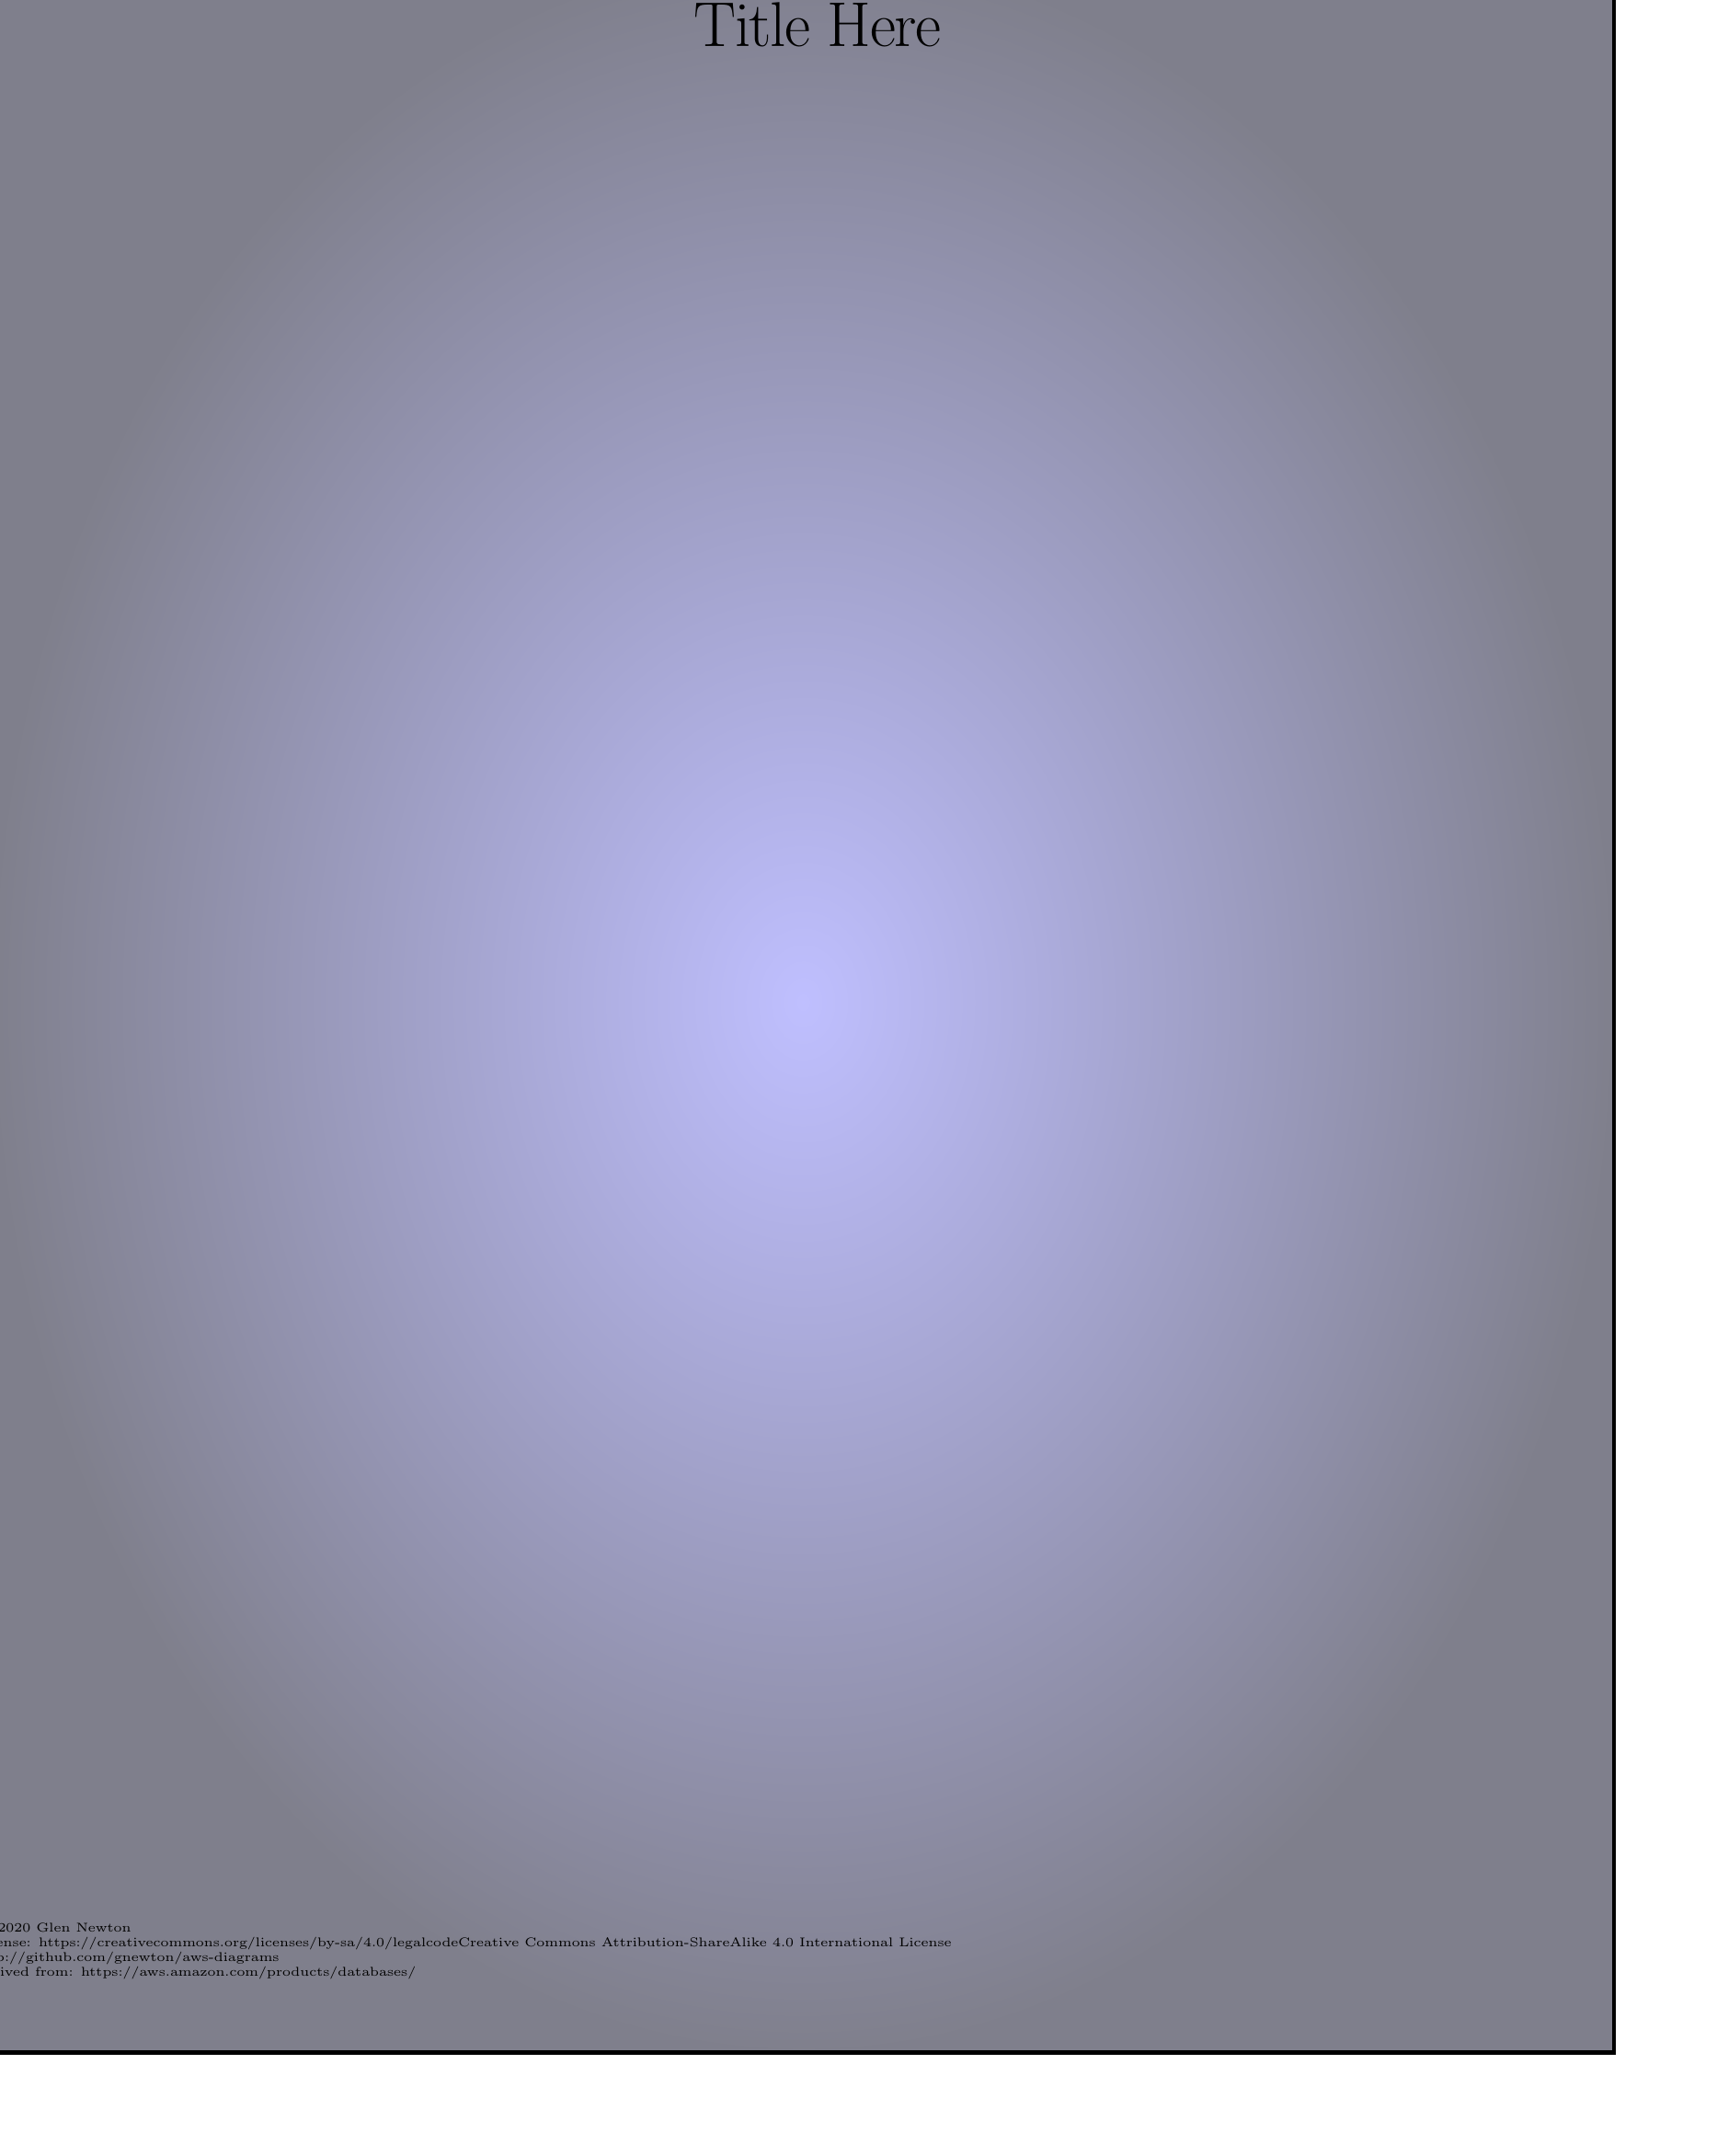
\begin{tikzpicture}
                  \begin{scope}
                    \draw [ultra thick, inner color=blue!50!,outer color=blue!10!black, fill opacity=0.5] (-11.4,-18) -- (11,-18) -- (11,11) -- (-11.4,11) -- (-11.4,-18);
                  \end{scope}
                  \begin{scope}

                  \end{scope}
                  \node[xshift=0cm,yshift=10cm](title) {
                    \Huge Title Here
                    };
                  \node[xshift=-4.9cm,yshift=-16.5cm](foox) {
                    %                  Copyright 2020 Glen Newton
                                      \tiny
                  \begin{tabular}{l}
                  \\
                    \copyright \ 2020 Glen Newton\\
                    License: \href{https://creativecommons.org/licenses/by-sa/4.0/legalcode}{Creative Commons Attribution-ShareAlike 4.0 International License}\\
                    \url{http://github.com/gnewton/aws-diagrams} \\
                    Derived from: \url{https://aws.amazon.com/products/databases/}
                  \end{tabular}

                  };
  \end{tikzpicture}}}\par}


\end{document}
